\chapter{Первые эксперименты с конструктором}


\section{Модуль переключателей}

\begin{center}
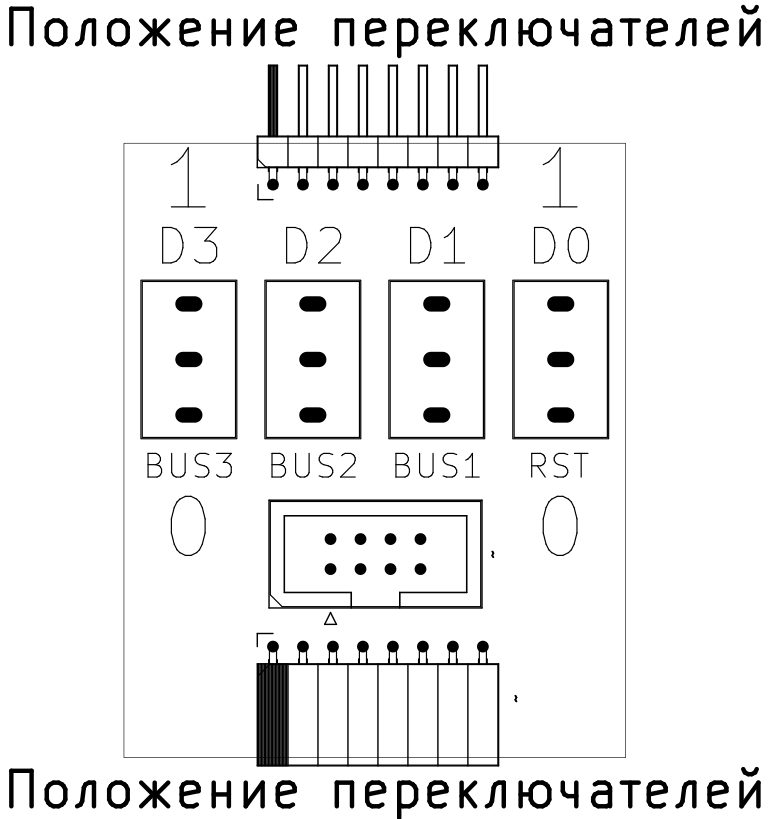
\includegraphics{boards/switches.png}
\end{center}

Модуль с тумблерами используется для ручного включения и выключения реле.
Присоединяя его к разным разъёмам, можно задавать четырёхбитное число,
либо переключать до четырёх управляющих сигналов.

Проще всего проверить работу тумблеров, подключив их к управляющей шине
регистрового модуля, в который вставлены только $4$ реле.

\subsection{Практикум}


Список модулей:
\begin{itemize}
    \item Модуль переключателей: $1$ штука
    \item Регистровый модуль как шинный формирователь: $1$ штука
\end{itemize}

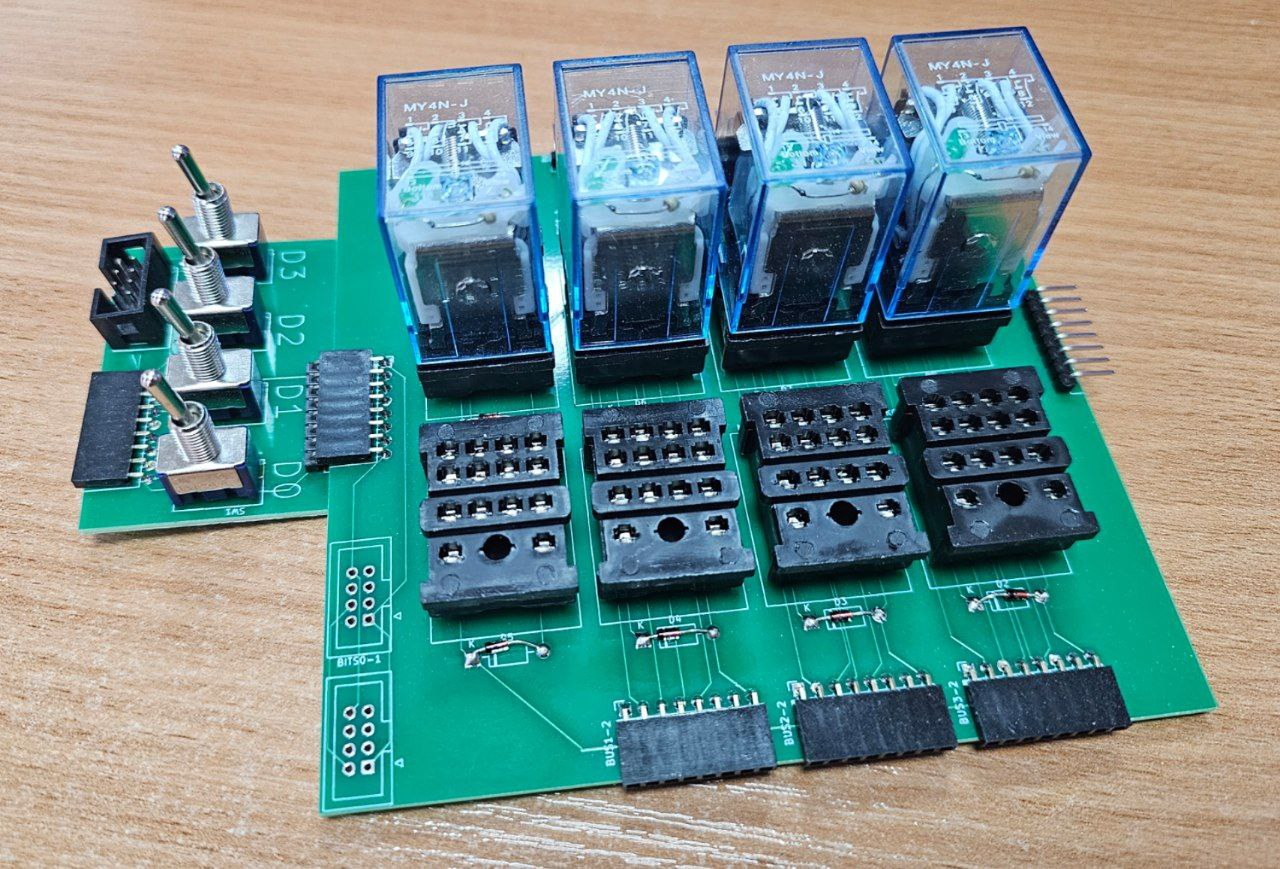
\includegraphics[width=0.5\columnwidth]{photo/switches.jpg}

\begin{enumerate}
    \item Переключать тумблеры. Убедиться, что положение одного тумблера меняет состояние одного реле.
    \item Запомнить включенное и выключенное состояния тумблера, чтобы позднее не было проблем с управлением другими схемами.
\end{enumerate}

\subsection{Задачи}

\begin{enumerate}
    \item Придумать, как соединить тумблеры для выполнения логического ИЛИ.
    \item Придумать, как соединить тумблеры для выполнения логического И.
\end{enumerate}
